\chapter{Concluding Remarks}
\label{chap:conclusion}

%\epigraph{
%\textit{When information is cheap, attention becomes expensive.}
%}
%{
%--James Gleick, \textit{The Information}
%}
%
%\epigraph{
%\textit{Our task as men is to find the few principles that will calm the infinite anguish
%of free souls. We must mend what has been torn apart, make justice imaginable again in a
%world so obviously unjust, give happiness a meaning once more to peoples poisoned by the
%misery of the century. Naturally, it is a superhuman task. But superhuman is the term
%for tasks men take a long time to accomplish, that's all.}
%}
%{
%--Albert Camus, \textit{The Almond Trees}
%}

\epigraph{
    \textit{The point is there ain't no point.}
}
{
    --Cormac McCarthy, \textit{No Country for Old Men}
}

%\epigraph{
%    \textit{The more the universe seems comprehensible, the more it also seems pointless.
%    But if there is no solace in the fruits of our research, there is at least some consolation
%    in the research itself. Men and women are not content to comfort themselves with tales of
%    gods and giants, or to confine their thoughts to the daily affairs of life; they also build telescopes
%    and satellites and accelerators, and sit at their desks for endless hours working out the meaning of the
%    data they gather. The effort to understand the universe is one of the very few things that lifts
%    human life a little above the level of farce, and gives it some of the grace of tragedy.}
%}
%{
%    --Steven Weinberg, \textit{The First Three Minutes}
%}

\epigraph{
    \textit{The effort to understand the universe is one of the very few things that lifts
    human life a little above the level of farce, and gives it some of the grace of tragedy.}
}
{
    --Steven Weinberg, \textit{The First Three Minutes}
}

%%%%%%%%%%%%%%%%%%%%%%%%%%%%%%%%%%%%%%%%%%%%%%%%%%%%%%%%%%%%%%%%%%%%%%%%%%%%%%%%%%%%%%%%%%%%%%
%%%%%%%%%%%%%%%%%%%%%%%%%%%%%%%%%%%%%%%%%%%%%%%%%%%%%%%%%%%%%%%%%%%%%%%%%%%%%%%%%%%%%%%%%%%%%%
%%%%%%%%%%%%%%%%%%%%%%%%%%%%%%%%%%%%%%%%%%%%%%%%%%%%%%%%%%%%%%%%%%%%%%%%%%%%%%%%%%%%%%%%%%%%%%

This dissertation has presented work related to the on-going upgrade of the forward muon system
of the ATLAS detector --- the New Small Wheel --- as well as two searches for BSM physics in dilepton final states.
The work thus described has taken place within the years 2015--2019, containing the entirety of the LHC Run 2,
and during a time of change in the physics program of the ATLAS experiment.

%%%%%%%%%%%%%%%%%%%%%%%%%%%%%%%%%%%%%%%%%%%%%%%%%%%%%%%%%%%%%%%%%%%%%%%%%%%%%%%%%%%%%%%%%%%%%%%%%%%%%%%%%%%%%%%%%%%%
%%%%%%%%%%%%%%%%%%%%%%%%%%%%%%%%%%%%%%%%%%%%%%%%%%%%%%%%%%%%%%%%%%%%%%%%%%%%%%%%%%%%%%%%%%%%%%%%%%%%%%%%%%%%%%%%%%%%
%%%%%%%%%%%%%%%%%%%%%%%%%%%%%%%%%%%%%%%%%%%%%%%%%%%%%%%%%%%%%%%%%%%%%%%%%%%%%%%%%%%%%%%%%%%%%%%%%%%%%%%%%%%%%%%%%%%%
%
% NSW
%
%%%%%%%%%%%%%%%%%%%%%%%%%%%%%%%%%%%%%%%%%%%%%%%%%%%%%%%%%%%%%%%%%%%%%%%%%%%%%%%%%%%%%%%%%%%%%%%%%%%%%%%%%%%%%%%%%%%%
%%%%%%%%%%%%%%%%%%%%%%%%%%%%%%%%%%%%%%%%%%%%%%%%%%%%%%%%%%%%%%%%%%%%%%%%%%%%%%%%%%%%%%%%%%%%%%%%%%%%%%%%%%%%%%%%%%%%
%%%%%%%%%%%%%%%%%%%%%%%%%%%%%%%%%%%%%%%%%%%%%%%%%%%%%%%%%%%%%%%%%%%%%%%%%%%%%%%%%%%%%%%%%%%%%%%%%%%%%%%%%%%%%%%%%%%%

At the time of writing in October 2019, the NSW project is on a critical path, at least with respect to its initial timeline of
being fully constructed and installed in ATLAS within the Phase 1 upgrade (c.f. Figure~\ref{fig:lhc_schedule}).
In the past few years, the NSW project has seen significant delays.
The construction of large-scale MM and sTGC detectors has never been done prior to the NSW, and
understanding the construction and behavior of these detectors has been a challenging process
that has, at times, required halting chamber production in order to understand emergent phenomena
that had not been foreseen.
The entire suite of frontend electronics has seen issues, as well, with one of the predominant issues being related to the
design of the ASICs themselves.
The important readout ASIC, the VMM, has had to go through at least one unforeseen design fix to address subtle
issues discovered in the lab, for example.
Even at the time of writing, the current understanding of the yield\footnote{The term `yield' here means
the fraction of produced VMMs that meet the performance criteria for being sufficient for use in ATLAS, and are not
failing specific criteria that are necessary in order to meet the physics goals of ATLAS.}
of the latest version of the VMM ASIC production is unknown.
Understanding this is currently of the utmost priority, since the frontend board development and construction of
detector chambers rely first on their being VMMs on-hand before they themselves can move forward and be fully commissioned.
If this yield is too low, additional ASICs will have to be manufactured at the silicon foundries, which is a lengthy (and expensive) process.
Additionally, the NSW will be the first major detector subsystem of ATLAS to use the upgraded TDAQ system based
on the Front-end Link Exchange (FELIX)~\cite{FELIX} backend.
FELIX, itself, has seen significant delays in its Phase 1 upgrade progress that have led to 
further slowing of the progress of the NSW.
With this in mind, the current best foreseen Phase 1 installation plan for the NSW project will be to install only a single wheel
into ATLAS before the start of LHC Run 3, with the second wheel being installed at some point
during Run 3, perhaps during one of the winter shutdown periods.
It may be likely that neither of the wheels is installed during Phase 1, at which point both will have to be scheduled
for installation in Run 3.
The NSW is a very ambitious project, and such issues as described here are not indicative of those
at the heart of moving it forward but rather a sign of the short window of time that such a large project
was aiming to be completed in, as well as its having started at a time of great busyness and distraction
at CERN.
% given that the start of the LHC and Higgs discovery happened so near the early days of the NSW project's start.
%had as its goal as well as its having started at a time of great busyness and distraction at CERN, what with the start
%of the LHC and Higgs discovery happening at the time that the NSW as a project was starting.
The current author looks forward to its complete commissioning and smooth operation within the ATLAS experimental cavern,
which will be a testament to many, many talented people from around the world having worked together
and designed, built, and butted-heads against a massive project of both new ideas and new technologies.


%%%%%%%%%%%%%%%%%%%%%%%%%%%%%%%%%%%%%%%%%%%%%%%%%%%%%%%%%%%%%%%%%%%%%%%%%%%%%%%%%%%%%%%%%%%%%%%%%%%%%%%%%%%%%%%%%%%%
%%%%%%%%%%%%%%%%%%%%%%%%%%%%%%%%%%%%%%%%%%%%%%%%%%%%%%%%%%%%%%%%%%%%%%%%%%%%%%%%%%%%%%%%%%%%%%%%%%%%%%%%%%%%%%%%%%%%
%%%%%%%%%%%%%%%%%%%%%%%%%%%%%%%%%%%%%%%%%%%%%%%%%%%%%%%%%%%%%%%%%%%%%%%%%%%%%%%%%%%%%%%%%%%%%%%%%%%%%%%%%%%%%%%%%%%%
%
% SUSY
%
%%%%%%%%%%%%%%%%%%%%%%%%%%%%%%%%%%%%%%%%%%%%%%%%%%%%%%%%%%%%%%%%%%%%%%%%%%%%%%%%%%%%%%%%%%%%%%%%%%%%%%%%%%%%%%%%%%%%
%%%%%%%%%%%%%%%%%%%%%%%%%%%%%%%%%%%%%%%%%%%%%%%%%%%%%%%%%%%%%%%%%%%%%%%%%%%%%%%%%%%%%%%%%%%%%%%%%%%%%%%%%%%%%%%%%%%%
%%%%%%%%%%%%%%%%%%%%%%%%%%%%%%%%%%%%%%%%%%%%%%%%%%%%%%%%%%%%%%%%%%%%%%%%%%%%%%%%%%%%%%%%%%%%%%%%%%%%%%%%%%%%%%%%%%%%

Given the naturalness arguments vying for electroweak-scale SUSY (Section~\ref{sec:susy}),
the most promising LHC signals for evidence of SUSY have been thought to be obtained in the searches for the direct production
of the stop quark, \stopone.
The search for the direct production of pairs of relatively light stops presented in this thesis provides a dilepton
strategy for thoroughly investigating this challenging phase space of SUSY, but has so far shown no signs of anything else
but consistency with the SM.
With the end of LHC Run 2, the SUSY searches for \stopone have generally designed analyses that can effectively
probe the \msn plane.
The analyses' strategies are therefore converging and are tending to be bound only by the available statistics
in the recorded data and center-of-mass collision energies.
Figure~\ref{fig:run2_stop_summary} shows the present status of all searches for the \stopone by ATLAS,
where it can be seen that present limits extend up to \stopone masses of 1 TeV.
Given the initial hopes for SUSY being `just around the corner' with the discovery of a relatively light Higgs boson,
the present limits extending to $m_{\stopone} \approx 1$\,TeV may seem disheartening to those who
have been `waiting in the wings', so to speak.
But one must remember the rather biased view of SUSY that such limits present, having been performed
under the hypotheses of simplified models of SUSY and with very specific instantiations of the MSSM.
In this light, it could be seen as being almost naive to consider searches for \stopone disheartening:
to have thought it promising in 2009, just as the LHC was turning on, and to think it less so now
is a rather impatient view of Nature~\cite{FengNaturalness}, especially given the many forms that the MSSM
can take while remaining consistent with a Higgs boson having a mass of 125 GeV~\cite{SUSYPrimer}.
Still, these last points bring skepticism to bear on the effectiveness of the direct searches for SUSY.
%Still, these last points bring to bear the effectiveness of the direct searches for SUSY.
At the very least, they motivate the continued push for the understanding of the most relevant
operating parameters of the MSSM such that searches with well-defined hypotheses can
be initiated.
Otherwise, the direct searches for the \stopone must be interpreted not as making statements
about SUSY, but rather as broad statements about the consistency between observation and prediction in extreme regions of phase space:
the SUSY simplified models only defining for the analyses topological handles with which metrics
quantifying their sensitivity to these kinematics and final states can be made.

\begin{figure}[!htb]
    \begin{center}
        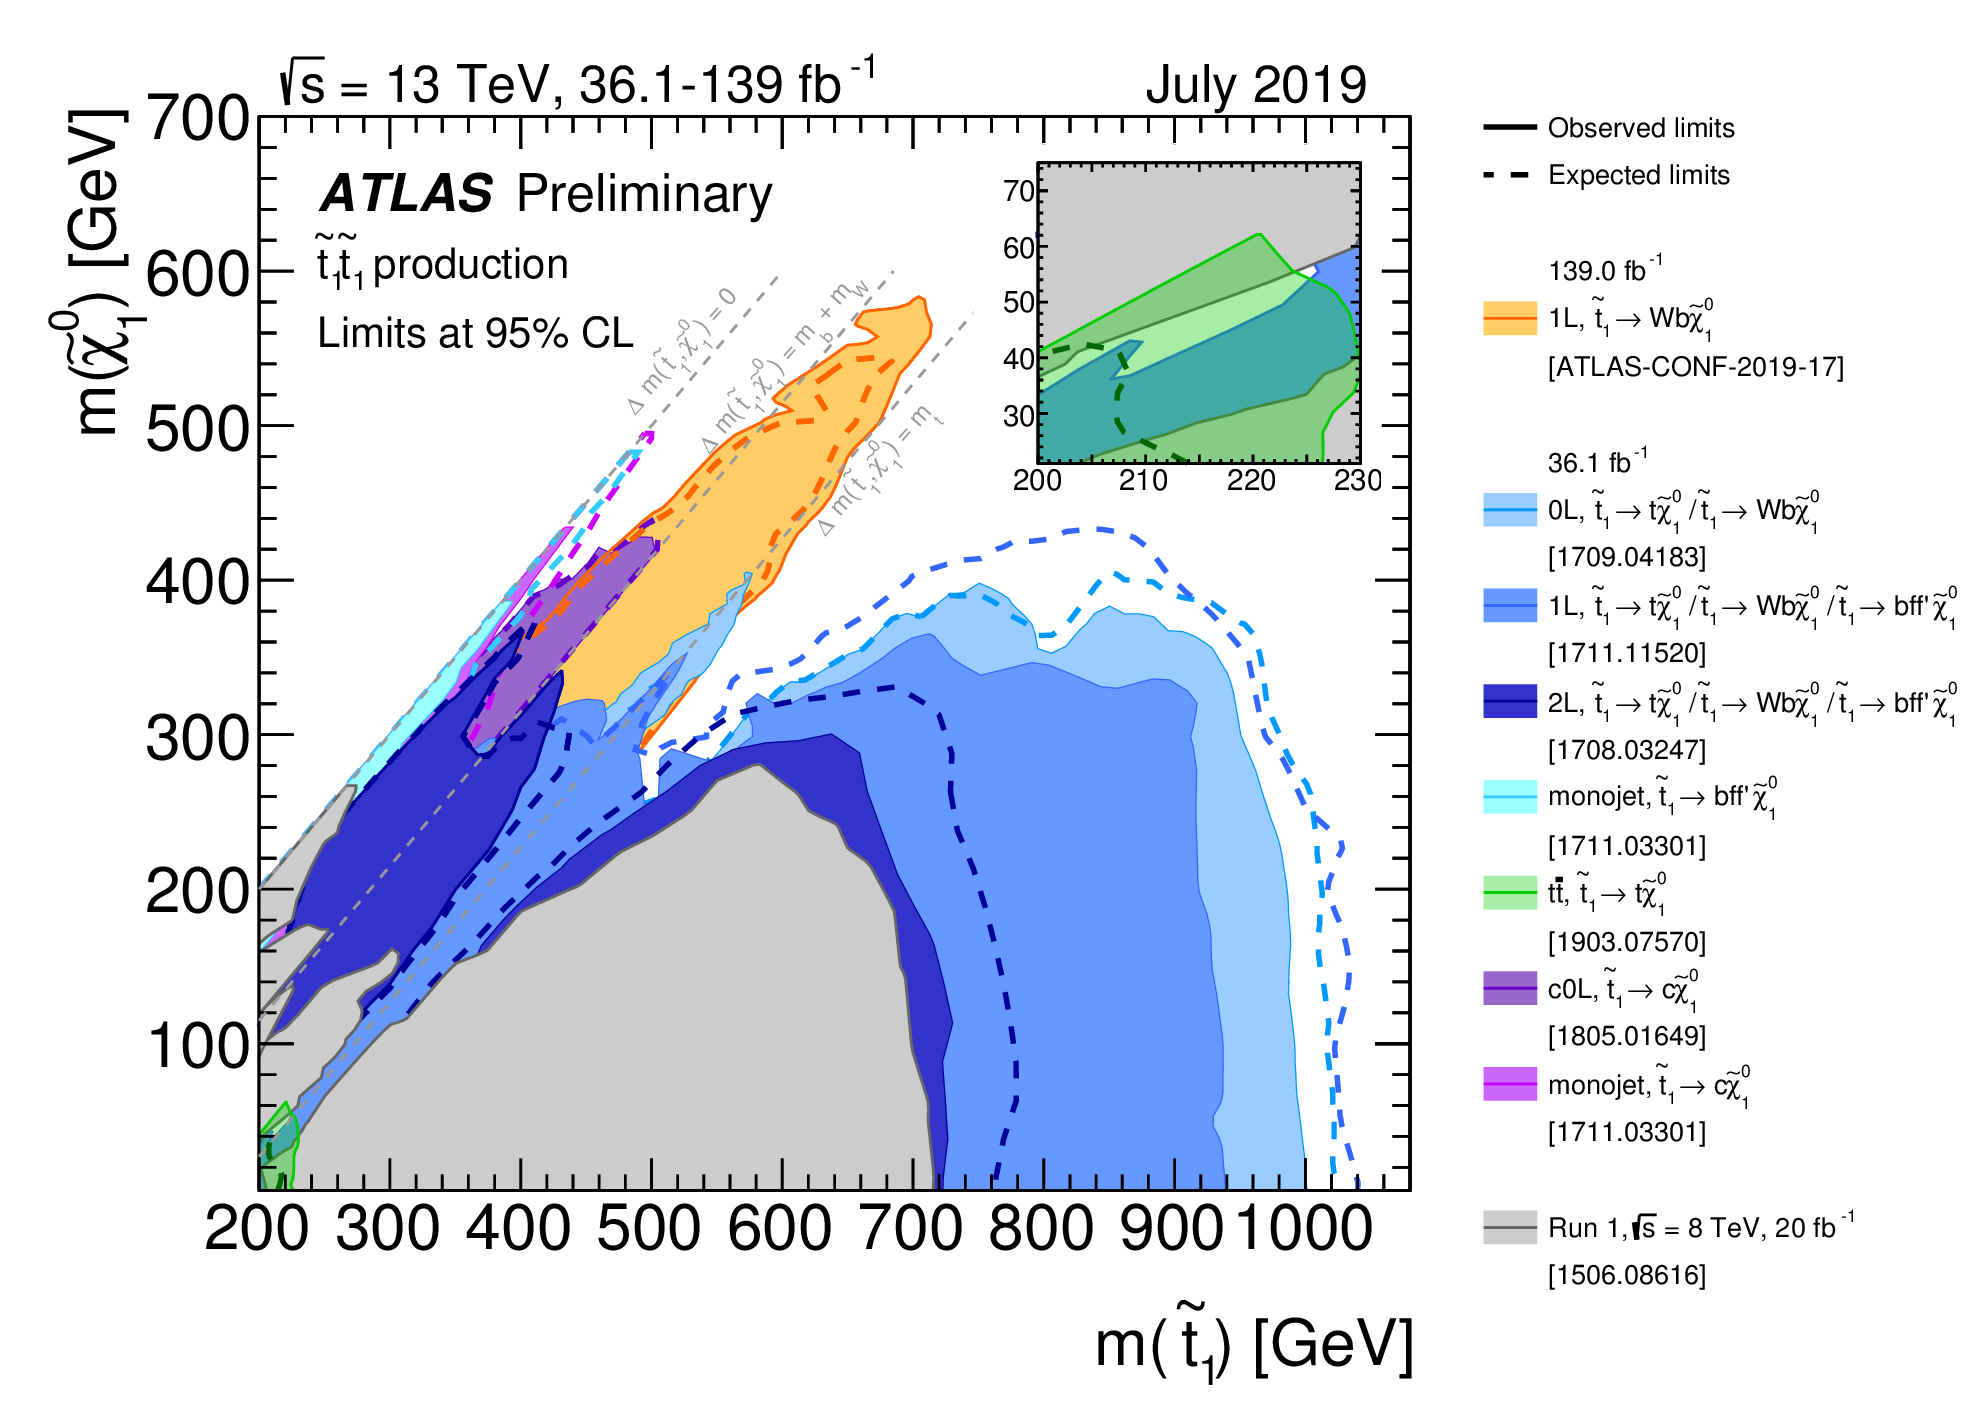
\includegraphics[width=0.85\textwidth]{figures/conclusion/ATLAS_SUSY_Stop_tLSP}
        \caption{
            Summary of ATLAS' LHC Run 2 exclusions in the $(\stopone, \ninoone)$ plane,
            as of July 2019.
        }
        \label{fig:run2_stop_summary}
    \end{center}
\end{figure}

%%%%%%%%%%%%%%%%%%%%%%%%%%%%%%%%%%%%%%%%%%%%%%%%%%%%%%%%%%%%%%%%%%%%%%%%%%%%%%%%%%%%%%%%%%%%%%%%%%%%%%%%%%%%%%%%%%%%
%%%%%%%%%%%%%%%%%%%%%%%%%%%%%%%%%%%%%%%%%%%%%%%%%%%%%%%%%%%%%%%%%%%%%%%%%%%%%%%%%%%%%%%%%%%%%%%%%%%%%%%%%%%%%%%%%%%%
%%%%%%%%%%%%%%%%%%%%%%%%%%%%%%%%%%%%%%%%%%%%%%%%%%%%%%%%%%%%%%%%%%%%%%%%%%%%%%%%%%%%%%%%%%%%%%%%%%%%%%%%%%%%%%%%%%%%
%
% HH
%
%%%%%%%%%%%%%%%%%%%%%%%%%%%%%%%%%%%%%%%%%%%%%%%%%%%%%%%%%%%%%%%%%%%%%%%%%%%%%%%%%%%%%%%%%%%%%%%%%%%%%%%%%%%%%%%%%%%%
%%%%%%%%%%%%%%%%%%%%%%%%%%%%%%%%%%%%%%%%%%%%%%%%%%%%%%%%%%%%%%%%%%%%%%%%%%%%%%%%%%%%%%%%%%%%%%%%%%%%%%%%%%%%%%%%%%%%
%%%%%%%%%%%%%%%%%%%%%%%%%%%%%%%%%%%%%%%%%%%%%%%%%%%%%%%%%%%%%%%%%%%%%%%%%%%%%%%%%%%%%%%%%%%%%%%%%%%%%%%%%%%%%%%%%%%%

With so many theories of BSM physics having something to say about the Higgs sector of the SM, mainly in their
having to address the Hierarchy Problem, the thorough study of this newly discovered particle
is of the utmost importance.
This is especially true in light of the failure of the direct searches for new physics to find any significant discrepancies
in the agreement of the observed data and the SM.
Towards this end, the ATLAS program for the search for the production of Higgs boson pairs is approaching
a level of maturity that will set itself up for the long-term LHC goal of observing this process.
It is only through the study of this process, and measurement of the Higgs boson self-coupling parameter, that a complete understanding of whether or not the Higgs sector behaves
as the SM predicts can be obtained.
The search presented in this thesis for SM-like Higgs boson pair production in the dilepton final state of $hh \rightarrow \bbww$
is a brand new addition to this search program, having filled a gap in the $hh$ searches' coverage that had
been previously disregarded for one reason or another.
%The dilepton $hh \rightarrow \bbww$ analysis described here is the first iteration of this search and appears to already be competitive with those search channels
It is the first iteration of this search; however, it appears to already be competitive with those search channels
previously thought to be the only means of being sensitive to the $hh$ production process.
That said, there is much to be improved with the analysis, as touched upon in Chapter~\ref{chap:search_hh}.
In the lead up to --- and during --- Run 3,
as the dilepton $\bbww$ channel becomes more well understood,
it will likely become more relevant to the overall search for the $hh$ process and in its ability
to constrain BSM effects in the Higgs sector that would act to modify the $hh$ production cross-section
or to alter the Higgs boson self-coupling parameter.
If meaningful statements about the underlying nature of EWSB
%If meaningful statements about these quantities and a better understanding of the underlying nature of EWSB
are to be made by the end of the HL-LHC era,
these searches must be active areas of study and their optimality must be ensured as soon as possible.
If anything, the addition of a new search channel at the end of LHC Run 2 that was previously not thought to be
relevant has sparked a little extra momentum on this front.
